\chapter{Conceptos previos}

\section{Métodos Numéricos y Ecuaciones Diferenciales Ordinarias}

Una ecuación diferencial es aquella que relaciona una función ( $f(x)$ ó $y$), sus variables ($x$) y sus derivadas ( $f’(x)$, $dy/dx$ ó $y’$ ). Para resolver una ecuación diferencial se debe encontrar una función que satisfaga dicha ecuación.
Dentro de las ecuaciones diferenciales nos encontramos las ecuaciones diferenciales ordinarias, EDOs, que contienen derivadas respecto a una sola variable independiente. Más adelante nos centraremos en este tipo en particular. En oposición a éstas estarían las ecuaciones en derivadas parciales, en las que la función $f(x)$ depende de más variables independientes. \cite{Molero2007}

El orden de una ecuación diferencial equivale al orden de la mayor derivada que aparece en la ecuación. Además, será lineal cuando la variable dependiente y todas sus derivadas son de primer grado (no puede haber $f(x)^2$ ), y los coeficientes de la variable dependiente y sus derivadas dependen de la variable independiente.

A modo de ejemplo simple podríamos considerar una ecuación diferencial ordinaria de primer orden como:

\begin{equation}
	\frac{dy}{dt} = -2y \text{ , } y(0)=1
\end{equation}

Donde además de la EDO, se nos está dando su valor inicial. En este caso en particular, sabemos de forma analítica que su solución exacta es $y(t) = e^{-2t}$, y podríamos por tanto calcular cualquier $y(t_n)=y_n$ que deseemos. No obstante, si por cualquier razón no pudiéramos resolverla analíticamente deberíamos recurrir a los métodos numéricos. A través de ellos, y partiendo del valor $y_n$ que se nos proporciona, calcularíamos de forma iterativa $y(t_{n+h})$ hasta llegar al valor $t_n=t_f$ que busquemos como estado final. 

\textbf(DIBUJAR FIGURA AVANCE PASO A PASO)

Podríamos utilizar para EDOs con valor inicial, por ejemplo, el método de Euler, del que hablaremos más adelante. Antes de ello podemos entrar en algo más de detalle respecto a algunos otros conceptos que iremos usando. 


\section{Tipos de métodos numéricos}

Podemos dividir a los métodos en tres grupos, explícitos, implícitos y semiimplícitos. La división se hará en función de cómo se consigue el siguiente paso, es decir, de cómo obtenemos $y_{n+1}$ a partir de $y_n$; de si aparecen valores futuros o no en la fórmula que lo calcula. Tendremos como expresión general la siguiente: \cite{Molero2007}

\begin{equation}
	\label{eq:ExpresionGeneralMetodosUnPaso}
	y_{n+1} = y_n + \Delta t \cdot \Phi (x_n, y_n, y_{n+1}, \Delta t)
\end{equation}

En la cual será la función incremento $\Phi$ la que dirima a cuál de los grupos pertenece el método con el que estemos trabajando.

Los métodos explícitos son aquellos en los que siguiente término se puede obtener directamente, sólo haciendo cálculos con datos de los que ya se dispone. Dicho de otra forma, son aquellos en los que $y_{n+1}$ no aparece en $\Phi$, sólo aparece en la parte izquierda de la ecuación. Entre ellos nos encontraremos el Euler explícito, Runge-Kutta, o Adams-Bashforth, los tres los veremos posteriormente. Los métodos explícitos suelen ser más fáciles de implementar, ya que no requieren resolver ecuaciones, y suelen ser más rápidos. Por otro lado, tienden a ser menos estables, especialmente en problemas rígidos (\textit{stiff}).

Al otro lado del espectro nos encontraríamos a los métodos implícitos, que son aquellos en los que $y_{n+1}$ sí aparece en la parte de la derecha de la igualdad, lo cuál nos obligaría a resolver una ecuación que podrá ser, o no, lineal. Estos métodos son muy estables, y son más adecuados para resolver problemas rígidos (\textit{stiff}). Como parte negativa tienen que requieren resolver ecuaciones en cada paso, y a veces de forma iterativa, lo que los acaba haciendo mucho más costosos computacionalmente. Entre ellos nos encontramos algunos métodos como el Euler implícito, Adams-Moulton, o los métodos BDF. 

Como tercer grupo tendríamos los métodos semiimplícitos. Éstos representan una especie de "solución" a los diferentes problemas que traen consigo los métodos explícitos e implícitos. En este grupo, aunque existe una parte implícita, ésta es más simple, ya que o bien la ecuación a resolver es lineal, o bien se separa la parte rígida para tratarla implícitamente y el resto se trata de forma explícita. Esto es útil cuando el problema tiene términos rígidos (\textit{stiff}) como la difusión, que deben tratarse implícitamente para que el método sea estable incluso con pasos de tiempo grandes, y términos suaves o de comportamiento hiperbólico como la advección, que se pueden tratar explícitamente para evitar resolver sistemas grandes o no lineales.
Los métodos semiimplícitos representan un compromiso entre la estabilidad de los explícitos y la velocidad de los implícitos. Como hemos mencionado, podremos dividir a la EDO en dos partes:

\begin{equation}
	\label{eq:EcuacionSemiimplicita}
	y' = f(x,y) = f_E(x,y) + f_I(x,y)
\end{equation}

En este ejemplo $f_E$ es la parte explícita, suave (no \textit{stiff}), y $f_I$ es la parte que queremos tratar implícitamente. Algunos métodos semiimplícitos son los métodos IMEX (\textit{implicit-explicit})\cite{Ascher1995}, los métodos linealmente implícitos Runge-Kutta (\textit{LIRK})\cite{Calvo2001}, o el método Adams-Bashforth-Moulton (AB-AM predictor-corrector). Es con este último con el que trabajaremos. 

Otra categorización con la que trabajaremos serán los métodos de un solo paso, y los métodos multipaso.
En los métodos de un solo paso, para obtener el siguiente valor con el que se tratará, el siguiente paso, sólo se utiliza información relativa al paso anterior. Es decir, como podemos ver en \ref{eq:ExpresionGeneralMetodosUnPaso}, para obtener $y_{n+1}$ sólo se utilizaría $y_n$.

Sin embargo, los métodos multipaso usan varios valores anteriores de la solución para calcular el siguiente paso en el tiempo, en lugar de basarse solo en el valor actual. Es decir, que para obtener $y_{n+1}$ se podrían tomar pasos intermedios que posteriormente se desechen (como en Runge-Kutta), o utilizar pasos más antiguos como $y_{n-1}$ o $y_{n-2}$. Para problemas de gran tamaño, los métodos multipaso permiten alcanzar resultados con gran precisión y de una forma más eficiente que los métodos de un paso como el de Euler o el de Runge-Kutta.


\section{Método de Euler}

Como hemos comentado, el método de Euler es uno de los métodos numéricos más simples de los que disponemos para la resolución de EDOs. Se trata de un método explícito de un solo paso que se construye a partir de una sencilla idea geométrica: aproximar el valor de la solución en cada nodo por el valor que proporciona la recta tangente a la solución trazada desde el punto correspondiente al nodo anterior.\cite{Gallardo2018} 

\begin{figure}[H]
	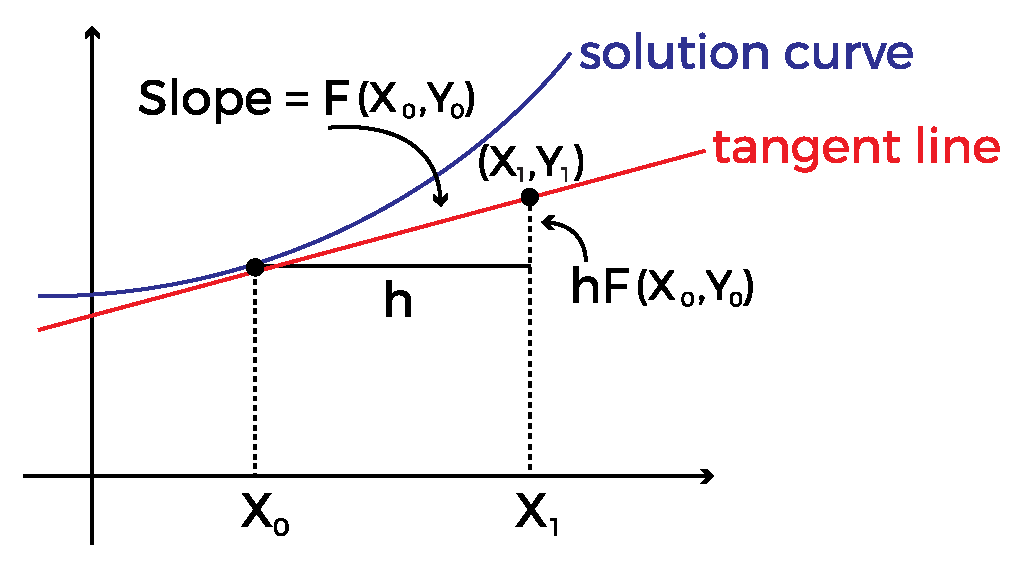
\includegraphics[width=\linewidth]{imagenes/Ejemplo-Euler.png}
	\caption{Aplicación del método de Euler \cite{Calcs2023}}
	\label{fig:Ejemplo-Euler}
\end{figure}

Emplearíamos la siguiente fórmula, aunque puede aparecer escrita de distintas formas equivalentes, aquí mostramos dos:

\begin{equation}
	\label{eq:EulerExplicito}
	\begin{split}
		y_{n+1} &= y_n + \Delta t \cdot f(t_n,y_n) \\
		y_{n+1} &= y_n + h \cdot f(x_n,y_n)
	\end{split}
\end{equation}

Aplicando la misma al ejemplo de valor inicial que mencionamos antes, $\frac{dy}{dt} = -2y \text{ , } y(0)=1$, sabemos que $y_n$ corresponde a la aproximación numérica de $y(t_n)$, y $\Delta t$ (o $h$) representa la variación en el tiempo paso a paso que estemos considerando. Además, en nuestro caso, $f(t_n,y_n)$ sería $-2 \cdot y_n$, y se nos da el valor inicial $t_0 = 0.0$. Por tanto, tomando estos valores, con un $\Delta t = 0.1$, y $t_f = 1.0$, calcularemos los sucesivos valores para $t = 0.1, 0.2, ..., 1.0$.

El primer paso sería por tanto, partiendo de los valores iniciales, calcular el $t=0.1$, a saber, $y_1 = y_0 + \Delta t \cdot f(t_0,y_0) = 1 + 0.1 \cdot (-2 \cdot 1) = 0.8 $. Si esto lo repitiéramos de forma sucesiva obtendríamos los siguientes resultados, los cuales además compararemos con el valor real $y(t) = e^{-2t}$ para obtener el error absoluto $\varepsilon_a$ y el error relativo $\varepsilon_r$. Definiremos al error absoluto como la diferencia entre el valor real y nuestra aproximación, y al error relativo como el cociente entre el error absoluto y el valor real, en porcentaje.

\begin{table}[H]
	\begin{center}
		\begin{tabular}{| c | c | c | c | c | c |}
			\hline
			Paso $n$ & $t_n$ & $y_n$(Euler) & $y_n$(Exacta) & $\varepsilon_a$ & $\varepsilon_r$ \\ \hline
			0  & 0.0 & \multicolumn{2}{c|}{Valor Inicial = 1.0} & - & - \\
			1  & 0.1 & 0.8     & 0.81873 & 0.01873 &  2.29 \\
			2  & 0.2 & 0.64    & 0.67032 & 0.03032 &  4.52 \\
			3  & 0.3 & 0.512   & 0.54881 & 0.03681 &  6.71 \\
			4  & 0.4 & 0.4096  & 0.44933 & 0.03973 &  8.84 \\
			5  & 0.5 & 0.32768 & 0.36788 & 0.04020 & 10.93 \\
			6  & 0.6 & 0.26214 & 0.30119 & 0.03905 & 12.97 \\
			7  & 0.7 & 0.20972 & 0.24660 & 0.03688 & 14.96 \\
			8  & 0.8 & 0.16777 & 0.20190 & 0.03412 & 16.90 \\
			9  & 0.9 & 0.13422 & 0.16530 & 0.03108 & 18.80 \\
			10 & 1.0 & 0.10737 & 0.13534 & 0.02796 & 20.66 \\ \hline
		\end{tabular}
		\caption{Comparativa entre Euler y valor real}
		\label{tab:Comparativa-Euler}
	\end{center}
\end{table}

\begin{figure}[H]
	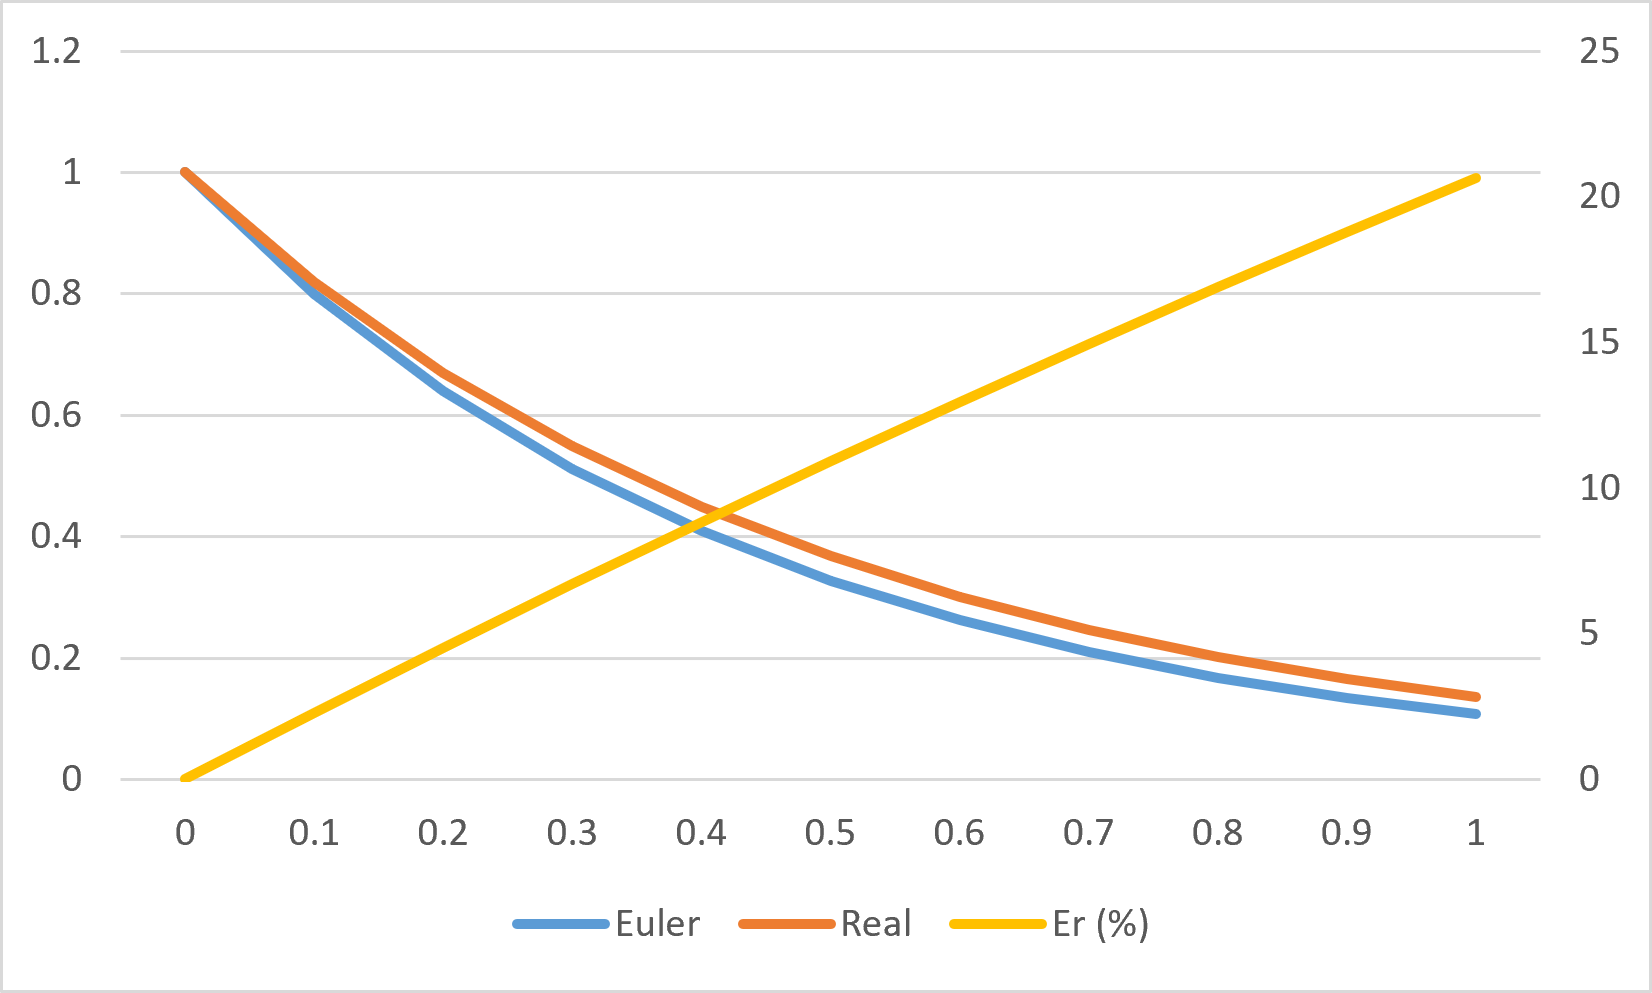
\includegraphics[width=\linewidth]{imagenes/Comparativa-Euler.png}
	\caption{Comparativa entre Euler y valor real}
	\label{fig:Comparativa-Euler}
\end{figure}

Como podemos observar en la tabla \ref{tab:Comparativa-Euler} y en la figura \ref{fig:Comparativa-Euler}, los valores que obtenemos con el Euler explícito son próximos a los reales (eje Y izquierdo); el error absoluto se mantiene estable por debajo de 0.05, e incluso disminuye. Sin embargo, el error relativo (eje Y derecho) aumenta de forma lineal con cada iteración, y para la última alcanza un preocupante 20\%. Esto nos indica que para este problema, quizás el método numérico que hemos utilizado o el $\Delta t$ que hemos considerado no son los más indicados. 

\section{Paralelismo}
Las dos tecnologías que vamos a utilizar para introducir el paralelismo en nuestro código y las mejoras que trae consigo son OpenMP y CUDA, es decir, paralelismo a  nivel de CPU, y a nivel de GPU, respectivamente.

Por muy rápida que sea nuestra CPU, siempre llegaremos a un punto en que, bien por la complejidad de los problemas, bien por el tamaño que se maneje, una sola CPU con un código secuencial no va a ser suficiente. Es aquí donde entra el paralelismo, y es aquí donde nos centraremos.

La programación paralela es el conjunto de técnicas, modelos y arquitecturas que permiten ejecutar múltiples operaciones de forma simultánea, explotando el hardware moderno (CPU multicore, GPU masivamente paralelas, aceleradores, clústeres). Su objetivo es reducir el tiempo de ejecución, aumentar el rendimiento y permitir resolver problemas que, como hemos comentado, serían inviables en código secuencial.

El paralelismo surge cuando un problema puede descomponerse en subtareas independientes que pueden ejecutarse al mismo tiempo. En términos formales, un programa es paralelizable si existe una partición de su espacio de trabajo en unidades que no presentan dependencias de datos que impidan su ejecución concurrente. Esto implica analizar dependencias de datos, localidad y acceso a memoria, granularidad de las tareas, y coste de sincronización.

Podríamos clasificar los distintos modelos de paralelismo que nos encontraremos de la siguiente forma. Por un lado tendríamos el paralelismo de datos, que consiste en aplicar la misma operación a múltiples elementos de un conjunto, a través de la vectorización, de bucles paralelos, o de operaciones \textit{element-wise}. Dentro de esta categoría nos encontraríamos a OpenMP, CUDA, OpenCL, o AVX, entre otros.

Por otro lado tendríamos el paralelismo de tareas, que consiste en ejecutar tareas heterogéneas en paralelo, como pipelines, árboles de tareas, o grafos de dependencias. Este modelo es usado por frameworks como TBB, Cilk, OpenMP tasks o runtimes de grafos. Por último el paralelismo híbrido combina ambos, buscando el paralelismo de tareas, con paralelismo de datos dentro de cada tarea.

Algunos conceptos muy importantes que nos encontraremos son la concurrencia y el paralelismo. La concurrencia hace referencia a que varias tareas pueden ocurrir a la vez, o que ocurren simultáneamente de forma lógica. Una CPU \textit{single-core} puede cambiar rápidamente de una tarea a otra si no tienen dependencia entre ellas y son concurrentes. Mientras que el paralelismo trata sobre ejecutar físicamente varias tareas al mismo tiempo, por ejemplo a través de varios núcleos (como en OpenMP) o de varias hebras (como en CUDA).

El speedup será la forma en la que mediremos las mejoras en la ejecución conforme aumenta el paralelismo. En nuestro caso, lo calcularemos dividiendo el tiempo de ejecución del programa secuencial, entre el paralelizado.\cite{Schryen2024} Como todo código por bien optimizado que esté va a tener una parte secuencial que no pueda paralelizarse, buscaremos que el speedup aumente tanto como sea posible. Por ejemplo, pasando de un código secuencial a uno con 4 hebras OpenMP, el speedup ideal sería de 4, aunque entendemos que no será posible conseguirlo, pero sí acercarse lo suficiente. 

Otro concepto relacionado sería el de la eficiencia, que sería el cociente entre speedup y el número de cores, o de hebras, empleado para obtener ese speedup. La eficiencia estará entre 0 y 1 (o entre 0\% y 100\%), y medirá cuánto se están aprovechando los recursos paralelos.

Al hilo de esto último, la Ley de Amdahl \cite{Amdahl1967} nos indica que, con un tamaño de problema constante y aumentando el número de procesadores, la parte no paralelizable del programa va a limitar nuestro speedup. Podemos ilustrarla tal que:

\begin{equation}
	\label{eq:LeyAmdahl}
	S(p) = \frac{1}{ (1-f) + f/p }
\end{equation}

Siendo $p$ el numero de procesadores, $f$ la fracción paralelizable del programa, $1-f$ por tanto sería la parte secuencial, y $S(p)$ sería el speedup máximo teórico. La interpretación que podemos hacer es que cuando aumentan los hilos, la parte no paralelizable satura el speedup. Por ejemplo, con un 95\% del programa paralelizable, e infinitos procesadores, el speedup nunca superará 20. Trayendo esto a un contexto más realista, lo que se nos indica es que, aunque obviamente aumentar los núcleos o los hilos es efectivo, y reduciremos los tiempos de ejecución, llegará un número a partir del cual ya no merezca la pena.

También debemos mencionar la Ley de Gustafson \cite{Gustafson1988}, que parte de una premisa distinta, aumentar el tamaño del problema cuando tenemos más procesadores. A saber:

\begin{equation}
	\label{eq:LeyGustafson}
	S(p) = p - (1-f) \cdot (p-1)
\end{equation}

Aquí la interpretación que hacemos es que al aumentar el tamaño del problema, aumentamos la parte paralelizable, mientras que la secuencial se mantiene estable. Esto juega a nuestro favor, ya que trataremos grandes cantidades de datos. La ley de Gustafson aporta un punto de vista más optimista al binomio procesadores-eficiencia, ya que nos dice que aunque la eficiencia no pueda ser perfecta, a medida que el problema y los hilos crezcan, podrá acercarse mucho.

Otro concepto importante será el de la sincronización. Cuando hilos diferentes deban compartir algún dato entre ellos, o necesiten que haya terminado cierta tarea antes de empezar la siguiente, deberá haber una barrera en la que los hilos se esperen entre ellos. Estas barreras ralentizan mucho la ejecución y se deberá intentar reducirlas tanto como sea posible.